\section{Categorical and Conditional Parameters}

%\begin{frame}[c]{Categorical and Conditional Parameters}
%\framesubtitle{Introduction}
%\begin{itemize}
%    \item<+->{Our parameter configuration space $\pcs$ can possibly contain:
%    \begin{itemize}
%        \item<+->{Neural Network Architectures.}
%        \item<+->{Model-specific parameters.}
%        \item<+->{General optimization parameters.} 
%    \end{itemize}
%    }
%    \item<+->{Consider searching through such a space of parameters. Is every individual dimension of this search space-
%    \begin{itemize}
%        \item<+->{Continuous?}
%        \item<+->{Relevant?}
%    \end{itemize}
%    }
%\end{itemize}
%\end{frame}
%-----------------------------------------------------------------------
%\begin{frame}[c]{Categorical and Conditional Parameters}
%\framesubtitle{Categorical Parameters}
%\begin{itemize}
%    \item<+-> Parameters that draw values from a discrete domain instead of a real-valued domain.
%    \item<+-> Mathematically, a parameter $\hyperparam$ is a categorical parameter if $\hyperparam\in P$, where $P=\{p_1, p_2, \dots\}$ is a set of finite, discrete values.
%    \item<+-> Examples:
%    \begin{itemize}
%        \item<+-> For training a neural network, we may choose one flavor of SGD out of $\{Vanilla, \,RMSProp, \,Adam\}$.
%        \item<+-> For a layer in a Multi-Layer Perceptron, we may choose one activation function out of $\{tanh, \,sigmoid, \,relu, \,unit\}$.
%    \end{itemize}
%    \item<+-> Categorical parameters present a challenge: inferring gradients is not possible for unordered categories!
%    \item<+-> Another challenge: Each individual category, or possible value of a categorical parameter, contributes to the curse of dimensionality in naive search approaches.
%\end{itemize}
%\end{frame}
%%-----------------------------------------------------------------------
\begin{frame}[c]{Categorical and Conditional Parameters}
\framesubtitle{Hamming Distance Kernel}
\begin{center}
Placeholder - Describe Hamming Distance Kernel from Frank's PhD thesis, include visualization
\end{center}
\end{frame}
%-----------------------------------------------------------------------
%\begin{frame}[c]{Categorical and Conditional Parameters}
%\framesubtitle{Conditional Parameters}
%\begin{itemize}
%    \item<+-> Some parameters in the search space are only relevant in the context of specific values of other parameters.
%    \item<+-> For example, if we are training a Neural Network using SGD, the momentum parameter is only relevant when using a flavour of SGD that supports it, such as Adam,
%    \item<+-> Such parameters can be used to define conditional dependencies between parameters
%    \item<+-> These dependencies define active/inactive sub-spaces within the search space
%    \item<+-> Conditional parameters are most recognizable in the context of categorical parameters, but they need not be categorical
%    \item<+-> Similar to categorical parameters, inferring gradients is not possible due to the presence of active/inactive sub-spaces
%\end{itemize}
%\end{frame}
%-----------------------------------------------------------------------
\begin{frame}[c]{Categorical and Conditional Parameters}
\framesubtitle{Structured Search Spaces}
\begin{itemize}
    \item<+-> In HPO, we have prior knowledge about when some parameters in the search space are completely irrelevant
    \item<+-> Naively searching over the entire search space while disregarding any conditional dependencies is inefficient
    \item<+-> We can impose a structure over the search space with the help of conditional dependencies between the various parameters to speed-up and optimize the HPO task
\end{itemize}
\end{frame}
%-----------------------------------------------------------------------
\begin{frame}[c]{Categorical and Conditional Parameters}
\framesubtitle{Structured Search Spaces}
\begin{center}
    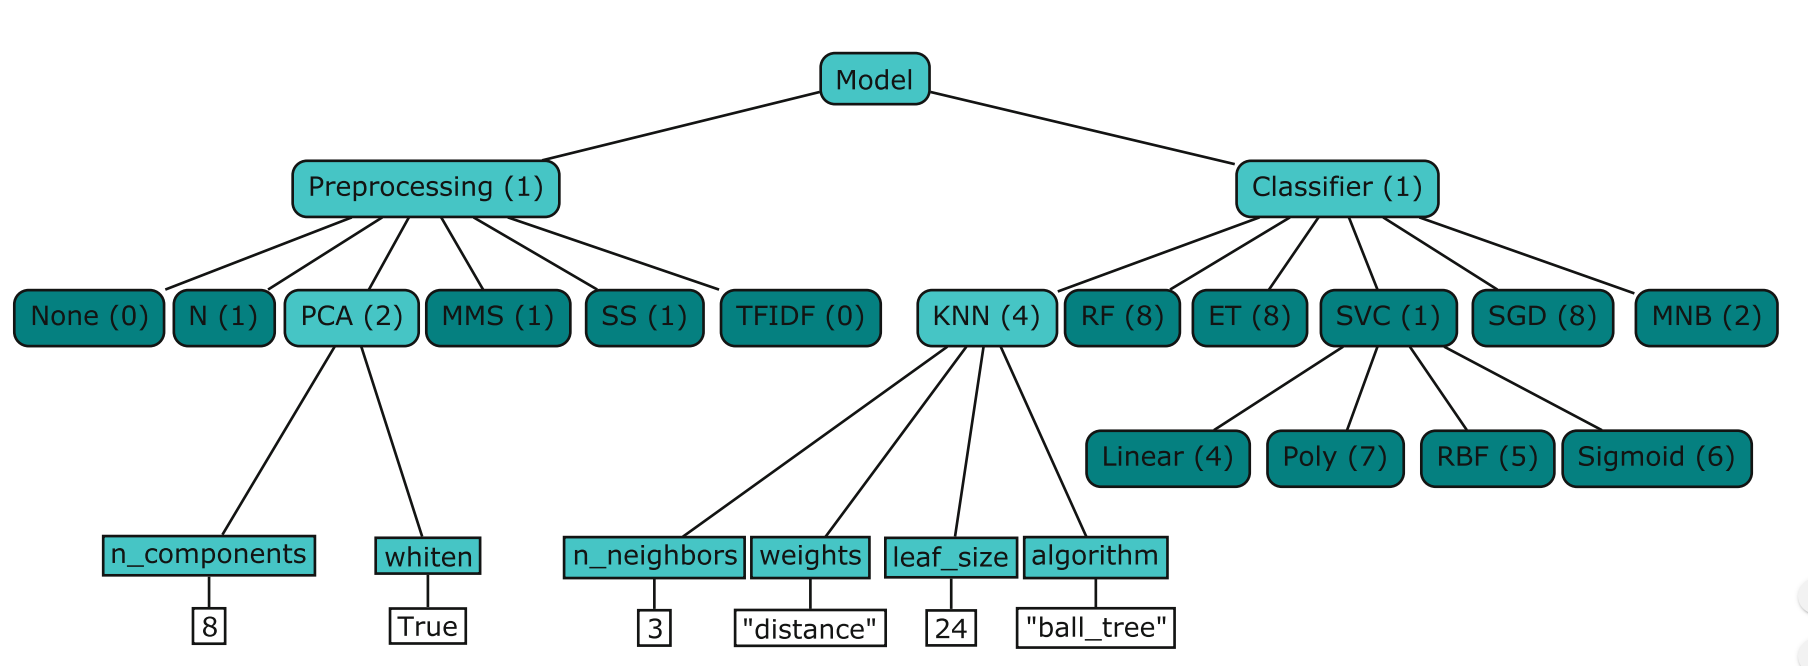
\includegraphics[width=.9\linewidth, height=0.9\textheight, keepaspectratio=true]{images/categ_cond_params/Conditional Parameters AutoML Book.png}
    \newline
    Example of a structured search space \comment{Source: Fig. 5.1 of the AutoML book}
\end{center}
\end{frame}
%-----------------------------------------------------------------------
\begin{frame}[c]{Categorical and Conditional Parameters}
\framesubtitle{Literature}
\begin{center}
    Placeholder
\end{center}
\end{frame}
%-----------------------------------------------------------------------